\section{Optimizaciones}

Las optimizaciones se han llevado a cabo sobre las funciones
\texttt{electric\_field} y \texttt{pythagoras}.

Las optimizaciones se han realizado de forma incremental. Esto significa que la
optimizaci\'{o}n X incluye las optimizaciones 0 a X-1 y que las modificaciones
se han realizado sobre la versi\'{o}n X-1.

El an\'{a}lisis de rendimiento de una optimizaci\'{o}n se ha hecho comparando
con la optimizaci\'{o}n anterior y con el c\'{o}digo de base. Con estas dos
comparaciones se puede observar cual es la ganancia total acumulada y la
ganancia de la optimizaci\'{o}n propuesta, respectivamente.

\subsection{Opt1: Evitar llamadas a funciones}

Las llamadas a funciones son un tipo de instrucci\'{o}n costosa que conviene
evitar siempre que sea posible. Algunas de las t\'{e}cnicas m\'{a}s comunes
para evitar llamadas a funciones son el inlining, la memorizaci\'{o}n o la
substituci\'{o}n de la llamada por un valor igual al valor de retorno.
\'{E}sta \'{u}ltima t\'{e}cnica es la que se puede utilizar para evitar llamar
a la funci\'{o}n \texttt{gaddress}.

La funci\'{o}n \texttt{gaddress} se encarga de calcular un \'{i}ndice de un
vector a partir de los cuatro par\'{a}metros que recibe. En el c\'{o}digo de
\texttt{electric\_field} se llama a la funci\'{o}n \texttt{gaddress} en
muchas ocasiones de forma innecesaria. La llamada es innecesaria porque la
secuencia de valores de retorno que generan las llamadas a \texttt{gaddress}
en el c\'{o}digo original es 0, 1, 2, ..., grid\_size-1, grid\_size+2,
grid\_size+3, etc. El c\'{o}digo original es el siguiente:

\begin{lstlisting}[]
     for( x = 0 ; x < grid_size ; x ++ ) {
        for( y = 0 ; y < grid_size ; y ++ ) {
           for( z = 0 ; z < grid_size ; z ++ ) {
              grid[gaddress(x,y,z,grid_size)] = ...
           }
        }
     }
\end{lstlisting}

La optimizaci\'{o}n propuesta consiste en cambiar la llamada a
\texttt{gaddress} por un simple contador que se incrementa en uno en cada
iteraci\'{o}n sobre \texttt{z} y en dos en cada iteraci\'{o}n sobre
\texttt{y}, generando as\'{i} los \'{i}ndices correctamente. El c\'{o}digo
resultante es el siguiente:

\begin{lstlisting}[]
     i = 0;
     for( x = 0 ; x < grid_size ; x ++ ) {
        for( y = 0 ; y < grid_size ; y ++ ) {
           for( z = 0 ; z < grid_size ; z ++ ) {
              grid[i] = ...
              i++;
           }
           i += 2;
        }
     }
\end{lstlisting}

Esta optimizaci\'{o}n se ha aplicado de la misma forma en otros puntos, como en
\texttt{electric\_field\_zero\_core} o en el primer bucle de
\texttt{electric\_point\_charge}.

\begin{figure}[ht]
   \centering
   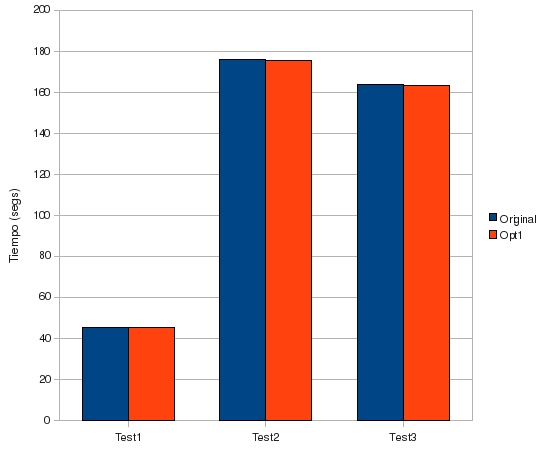
\includegraphics[keepaspectratio=true,width=.6\textwidth]{figures/opt1-perf}
\end{figure}

Aceleracion inicial	100.2886%	100.1491%	100.2726%

\subsection{Opt2: Filtrado de datos}

Explicar tecnica.

La primera l\'{i}nea del cuerpo del bucle es una comprobaci\'{o}n de que un
cierto valor es distinto de cero, pero lo cierto es que la comprobaci\'{o}n es
in\'{u}til. Si el valor es distinto de cero, se hacen una serie de c\'{a}lculos
y se acumula sobre una variable el resultado de dividir el valor por el
resultado de los c\'{a}lculos.

\begin{lstlisting}[]
     if( This_Structure.Residue[residue].Atom[atom].charge != 0 ) {
        ...
        phi += ( This_Structure.Residue[residue].Atom[atom].charge / ... ) ;
     }
\end{lstlisting}

Esta condici\'{o}n se puede eliminar ya que la ejecuci\'{o}n no cambia si
\texttt{This\_Structure.Residue[residue].\\Atom[atom].charge} es distinto de
cero y, si es cero, el resultado de divisi\'{o}n es cero y
\texttt{phi} se incrementa cero, haciendo que el resultado final sea correcto.
El problema es que el coste de hacer siempre este c\'{a}lculo es mayor que los
beneficios que supone ahorrarse la evaluaci\'{o}n de la condici\'{o}n y las
posibles penalizaciones
por fallos del predictor de saltos, as\'{i} que la eleminaci\'{o}n no se ha
llevado a cabo.

\begin{figure}[ht]
   \centering
   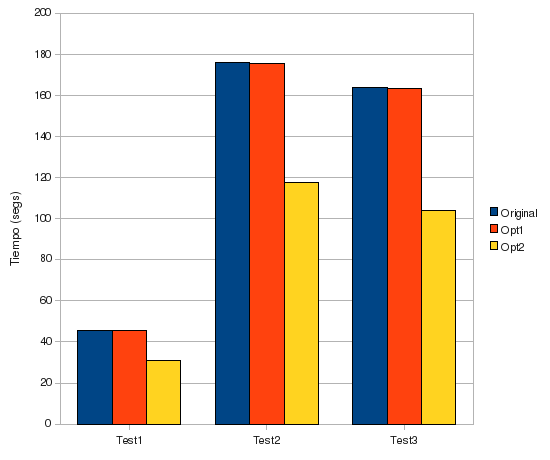
\includegraphics[keepaspectratio=true,width=.6\textwidth]{figures/opt2-perf}
\end{figure}


Aceleracion orig	147.7424%	149.8068%	157.5480%
Acelaracion prev	147.3172%	149.5838%	157.1197%

\subsection{Opt3: Evitar saltos}

Los saltos, como las llamadas a funciones, son instrucciones que pueden llegar
a ser muy costosas debido a  los posibles fallos del predictor de saltos, por
eso es conveniente evitar los saltos innecesarios.

En el bucle m\'{a}s interno de la funci\'{o}n \texttt{electric\_field} hay
varias comprobaciones que se traducen en saltos al compilar. Algunas de estas
comprobaciones son innecesarias u optimizables.

\begin{lstlisting}[]
     if( distance < 2.0 ) distance = 2.0 ;
     if( distance >= 2.0 ) {
        if( distance >= 8.0 ) {
           epsilon = 80 ;
        } else {
           if( distance <= 6.0 ) {
              epsilon = 4 ;
           } else {
              epsilon = ( 38 * distance ) - 224 ;
           }
        }
        phi += (This_Structure.Residue[residue].Atom[atom].charge/(epsilon*distance));
     }
\end{lstlisting}

La segunda comprobaci\'{o}n se puede eliminar ya que siempre se cumple debido a
la asignaci\'{o}n de la l\'{i}nea anterior. Adem\'{a}s, la secuencia de
condicionales imbricados para asignar un valor a \texttt{epsilon} se puede
simplificar. El c\'{o}digo resultante es:

\begin{lstlisting}[]
     if( distance < 2.0 ) distance = 2.0 ;
     if (distance >= 8.0)
        epsilon = 80;
     else if (distance <= 6.0)
        epsilon = 4;
     else
        epsilon = 38 * distance - 224;
     phi += (This_Structure.Residue[residue].Atom[atom].charge/(epsilon*distance));
\end{lstlisting}

Otra fuente de saltos innecesarios es el primer bucle de la funci\'{o}n
\texttt{electric\_field}. El c\'{o}digo original es:

\begin{lstlisting}
     i = 0;
     for( x = 0 ; x < grid_size ; x ++ ) {
        for( y = 0 ; y < grid_size ; y ++ ) {
           for( z = 0 ; z < grid_size ; z ++ ) {
              grid[i] = (fftw_real)0;
              i++;
           }
           i += 2;
        }
     }
\end{lstlisting}

Como se puede observar, los bucles sobre \texttt{x} e \texttt{y} se pueden
fusionar en uno solo y as\'{i} evitar un salto. El resulado es el siguiente
c\'{o}digo:

\begin{lstlisting}
     i = 0; 
     j = 0;
     while( j < grid_size*grid_size*grid_size) {
        for( i = j ; i < j+grid_size ; i ++ ) {
           grid[i] = (fftw_real)0;
        }
        j += grid_size + 2;
     }
\end{lstlisting}

Esta optimizaci\'{o}n se ha aplicado de la misma forma en otros puntos, como en
\texttt{electric\_field\_zero\_core} o en el primer bucle de
\texttt{electric\_point\_charge}.

\begin{figure}[ht]
   \centering
   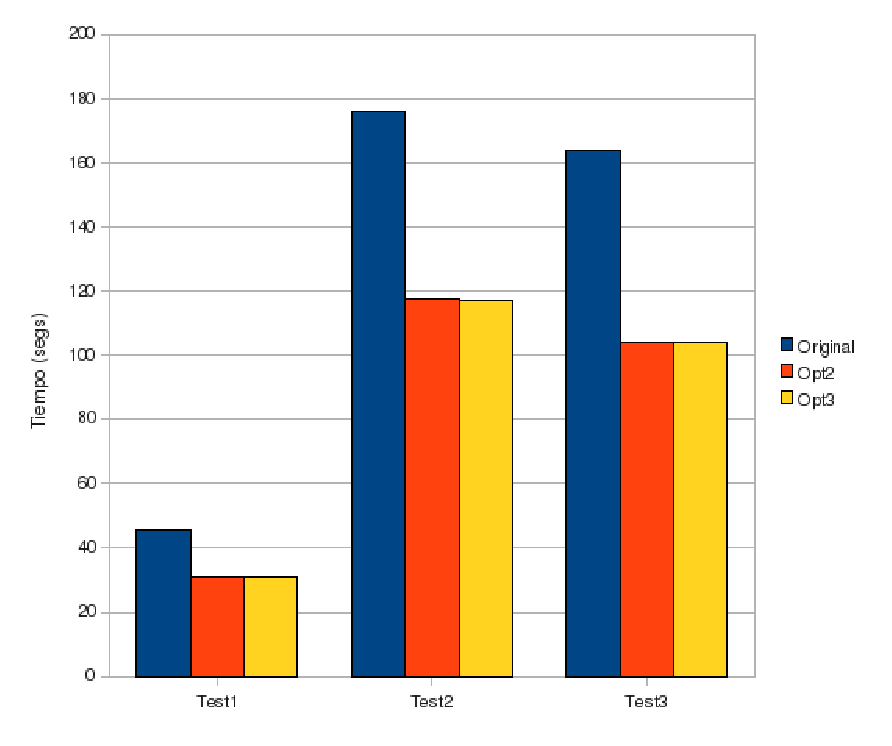
\includegraphics[keepaspectratio=true,width=.6\textwidth]{figures/opt3-perf}
\end{figure}

Aceleracion orig	148.0018%	149.9830%	157.6827%
Acelaracion prev	100.1756%	100.1176%	100.0855%

\subsection{Opt4: Evitar llamadas a sistema}

Las llamadas a sistema son un tipo de instrucci\'{o}n especialmente costoso, ya
que provocan tener que entrar a modo sistema, salvar el contexto, ensuciar la
cache, etc. La tecnica m\'{a}s utilizada para evitar llamadas a sistema es el
buffering, o juntar varias llamadas a sistema en una.

En cada iteraci\'{o}n del bucle m\'{a}s externo del cuerpo de
\texttt{electric\_field} se hace un \texttt{printf(".")}. Esto provoca que
la ejecuci\'{o}n se hagan \texttt{grid\_size} \texttt{printf}'s que escriben un
solo punto, cuando lo \'{o}ptimo es hacer un solo \texttt{printf} que escriba
\texttt{grid\_size} puntos.

\begin{figure}[ht]
   \centering
   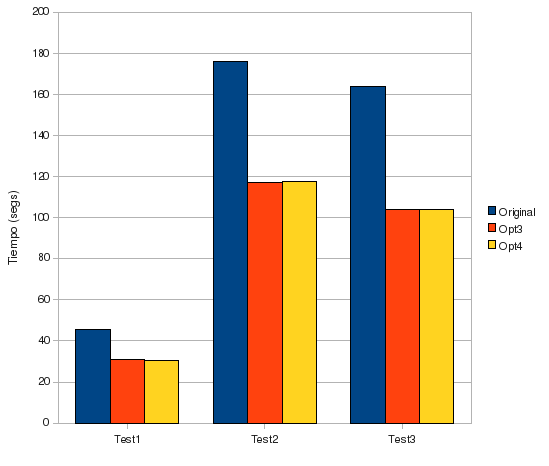
\includegraphics[keepaspectratio=true,width=.6\textwidth]{figures/opt4-perf}
\end{figure}

Aceleracion orig	148.3250%	149.8565%	157.8284%
Acelaracion prev	100.2183%	99.9157%	100.0924%

\subsection{Opt5: Unrolling}

El unrolling es una t\'{e}cnica que consiste en replicar el c\'{o}digo de un
bucle N veces para as\'{i} reducir el n\'{u}mero de saltos que se realizan al
ejecutar el c\'{o}digo de control del bucle. El n\'{u}mero de saltos se divide
por N.

En el c\'{o}digo original el bucle m\'{a}s interno se hace de esta forma:

\begin{lstlisting}
     for( atom = 1 ; atom <= This_Structure.Residue[residue].size ; atom ++ ) {
        cuerpo
     }
\end{lstlisting}

El unrolling realizado es de grado 4, es decir, se replica el cuerpo 4 veces y
se incrementa la variable \texttt{atom} en 4 en vez de en 1. Puede pasar que el
n\'{u}mero de iteraciones no sea divisible por 4, por eso hay que dividir el
bucle en dos. En el pre\'{a}mbulo se ejecutan iteraciones hasta que el
n\'{u}mero de iteraciones restante sea divisible por 4, y en el bucle principal
se hace el unrolling. El c\'{o}digo resultante es el siguiente:

\begin{lstlisting}
     num_non_unrolled_iters = This_Structure.Residue[residue].size % 4;
     for( atom = 1 ; atom <= num_non_unrolled_iters ; atom ++ ) {
        cuerpo
     }
     for( atom = 1 ; atom <= This_Structure.Residue[residue].size ; atom +=4 ) {
        cuerpo0
        cuerpo1
        cuerpo2
        cuerpo3
     }
\end{lstlisting}

\begin{figure}[ht]
   \centering
   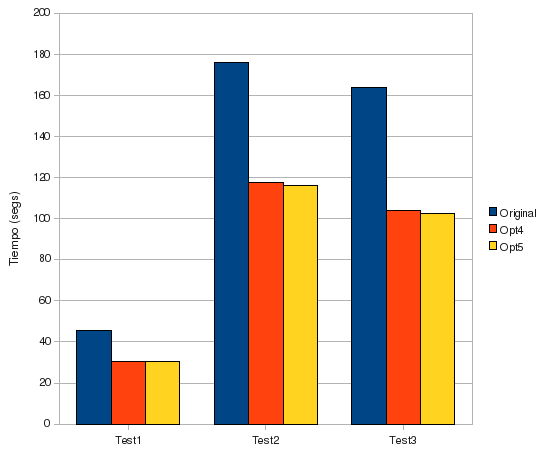
\includegraphics[keepaspectratio=true,width=.6\textwidth]{figures/opt5-perf}
\end{figure}

Aceleracion orig	149.9423%	151.2134%	159.9456%
Acelaracion prev	101.0904%	100.9055%	101.3415%

\subsection{Opt6: Vectorizaci\'{o}n}

Una vez el 

\begin{figure}[ht]
   \centering
   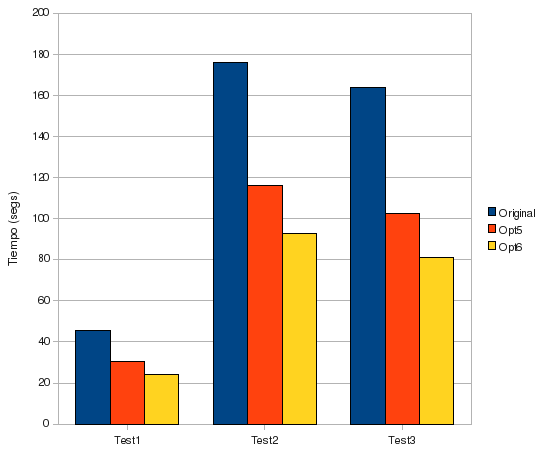
\includegraphics[keepaspectratio=true,width=.6\textwidth]{figures/opt6-perf}
\end{figure}

Aceleracion orig	187.6288%	189.7217%	202.4245%
Acelaracion prev	125.1340%	125.4662%	126.5583%

\subsection{Opt7: Vectorizaci\'{o}n}

En la funci\'{o}n \texttt{pythagoras} se calcula la distancia eucl\'{i}dea
entre dos vectores. Para calcularla se ejecutan muchas instrucciones: se restan
de componentes, se hacen tres exponencial cuadradas, se suman todas las
componentes y finalmente se hace una raiz cuadrada del resultado de la suma.

\begin{lstlisting}
	sqrt( 
		( ( x1 - x2 ) * ( x1 - x2 ) ) 
		+ 
		( ( y1 - y2 ) * ( y1 - y2 ) ) 
		+ 
		( ( z1 - z2 ) * ( z1 - z2 ) ) 
		) ;
\end{lstlisting}

La transformaci\'{o}n de esta funci\'{o}n a c\'{o}digo vectorial es inmediata:

\begin{lstlisting}
	__m128 v1 = _mm_set_ps(x1, y1, z1, 0);
	__m128 v2 = _mm_set_ps(x2, y2, z2, 0);
	
	v1 = _mm_sub_ps(v1, v2);
	v1 = _mm_mul_ps(v1, v1);
	
	_mm_storeu_ps(vector, v1);
	
	sqrt(vector[1]+vector[2]+vector[3]);
\end{lstlisting}

Como se puede ver en el codigo anterior, a la hora de cargar los valores al
registro vectorial hay que rellenar la \'{u}ltima posici\'{o}n con alg\'{u}n
valor aunque no se vaya a utilizar.

En este c\'{o}digo solo se hacen dos operaciones vectoriales, una suma y una
multiplicaci\'{o}n, adem\'{a}s de solo utilizar tres de los cuatro valores en
el registro vectorial. Estos dos motivos, junto con que para trabajar con
vectores se necesita hacer un load hacia el registro vectorial y un store a
memoria, hacen que empeore el rendimiento de la aplicaci\'{o}n.

\begin{figure}[ht]
   \centering
   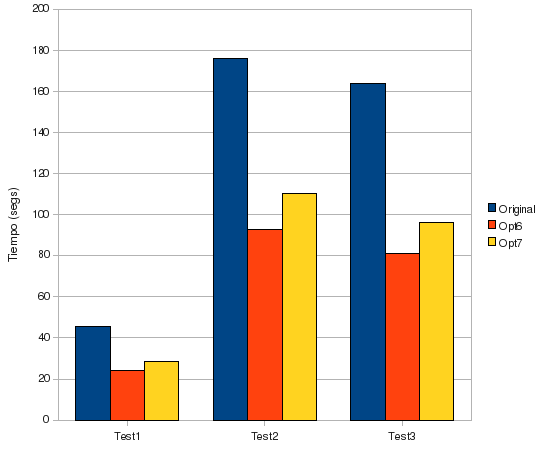
\includegraphics[keepaspectratio=true,width=.6\textwidth]{figures/opt7-perf}
\end{figure}

Aceleracion orig	158.1041%	159.2999%	170.4034%
Acelaracion prev	84.2643%	83.9650%	84.1812%

\subsection{Opt8: Vectorizaci\'{o}n con SSE3}

Para intentar solventar el problema del coste que tiene hacer un load y un store
a un registro vectorial para hacer solo dos operaciones se han a\~{n}adido
m\'{a}s operaciones vectoriales y se han eliminado los accesos a memoria
utilizando intr\'{i}nsicas de SSE3.

\begin{lstlisting}
	float result;
	
	__m128 v1 = _mm_set_ps(x1, y1, z1, 0);
	__m128 v2 = _mm_set_ps(x2, y2, z2, 0);
	
	v1 = _mm_sub_ps(v1, v2);
	v1 = _mm_mul_ps(v1, v1);

	v1 = _mm_hadd_ps(v1, v1);
	v1 = _mm_hadd_ps(v1, v1);
	v1 = _mm_sqrt_ss(v1);	
	
	_mm_store_ss(&result, v1);
\end{lstlisting}

Utilizado la intr\'{i}nseca \texttt{\_mm\_hadd\_ps} dos veces se ahorrarn las
sumas y la intr\'{i}nseca \texttt{\_mm\_sqrt\_ss} calcula la raiz cuadrada de la
suma anterior de forma muy eficiente. Esto, a\~{n}adido al hecho de tener que
recuperar solo un valor del registro vectorial, hace que el tiempo de
ejecuci\'{o}n mejore.

\begin{figure}[ht]
   \centering
   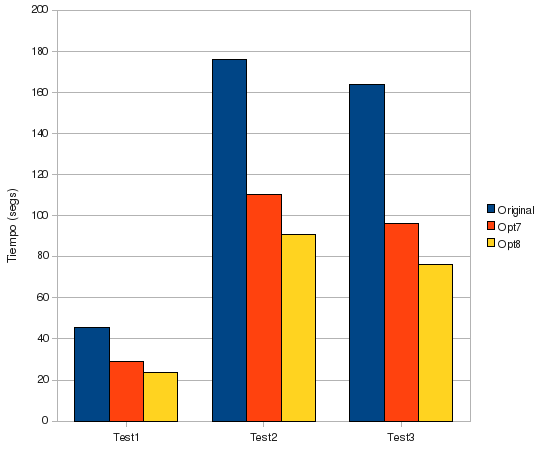
\includegraphics[keepaspectratio=true,width=.6\textwidth]{figures/opt8-perf}
\end{figure}

Aceleracion orig	191.2556%	193.7223%	215.7306%
Acelaracion prev	120.9681%	121.6086%	126.6000%

\subsection{Opt9: Inlining}

Viendo que el motivo principal de penalizaci\'{o}n en \texttt{pythagoras} son
los accesos a memoria y estudiando el or\'{i}gen de la mayor\'{i}a de las
llamadas a esta funci\'{o}n, se ha notado que hay parametros que se pasan a cada
llamada sin ser modificados. Este hecho provoca cargas al registro vectorial
innecesarias.

\begin{lstlisting}
	distance = pythagoras(This_Structure.Residue[residue].Atom[atom].coord[1], 
						  This_Structure.Residue[residue].Atom[atom].coord[2], 
						  This_Structure.Residue[residue].Atom[atom].coord[3],
						  x_centre, y_centre, z_centre);
\end{lstlisting}
 
Los valores \texttt{x\_centre}, \texttt{y\_centre} y \texttt{z\_centre} no
canbian a cada iteraci\'{o}n del bucle sin\'{o} que se mantienen constantes
durante muchas iteraciones. Por este motivo, haciendo inlining, se pueden
hacer cargas el registro vectorial solo cuando se modifica uno de estos valores.

\begin{lstlisting}
	z_centre  = gcentre( z , grid_span , grid_size ) ;
	__m128 v2 = _mm_set_ps(x_centre, y_centre, z_centre, 0);
	phi = 0 ;
	for( residue = 1 ; residue <= This_Structure.length ; residue ++ ) {
		for( atom = 1 ; atom <= This_Structure.Residue[residue].size ; atom ++ ) {
			if( This_Structure.Residue[residue].Atom[atom].charge != 0 ) {
				__m128 v1 = _mm_set_ps(This_Structure.Residue[residue].Atom[atom].coord[1],
						This_Structure.Residue[residue].Atom[atom].coord[2],
						This_Structure.Residue[residue].Atom[atom].coord[3], 0);
				v1 = _mm_sub_ps(v1, v2);
				v1 = _mm_mul_ps(v1, v1);
				v1 = _mm_hadd_ps(v1, v1);
				v1 = _mm_hadd_ps(v1, v1);
				v1 = _mm_sqrt_ss(v1);	
				_mm_store_ss(&distance, v1);
\end{lstlisting}

\begin{figure}[ht]
   \centering
   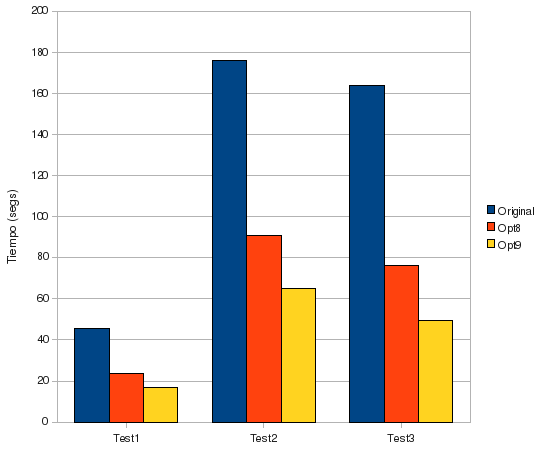
\includegraphics[keepaspectratio=true,width=.6\textwidth]{figures/opt9-perf}
\end{figure}

Aceleracion orig	266.7937%	271.4096%	332.8822%
Acelaracion prev	139.4959%	140.1024%	154.3046%

% vim: filetype=tex tw=75
